\chapter{User guide}

\section{Registration}
\label{sec:registration}

\subsection{Step 1}
The reimbursement-tool is connected to the UZH-IFI LDAP server. This allows employed persons at the IFI department to use their existing login credentials provided by the University of Zurich.\newline
On the initial login of a user he needs to pass a two-stepped registration process. On Figure \ref{fig:registration-step01} the user needs to input two values:
\begin{itemize}
    \item UZH personnel number is the employee number, written on the employment card. It is of the form \textit{01-123-456}. Enter the number without the leading 0 and hyphens; i.e. \textit{123456}.
    \item UZH phone number is the personnel phone number of the employee. Enter it in the form in the form \textit{0441234567}.
\end{itemize}


\begin{figure}[H]
    \centering
    \fbox{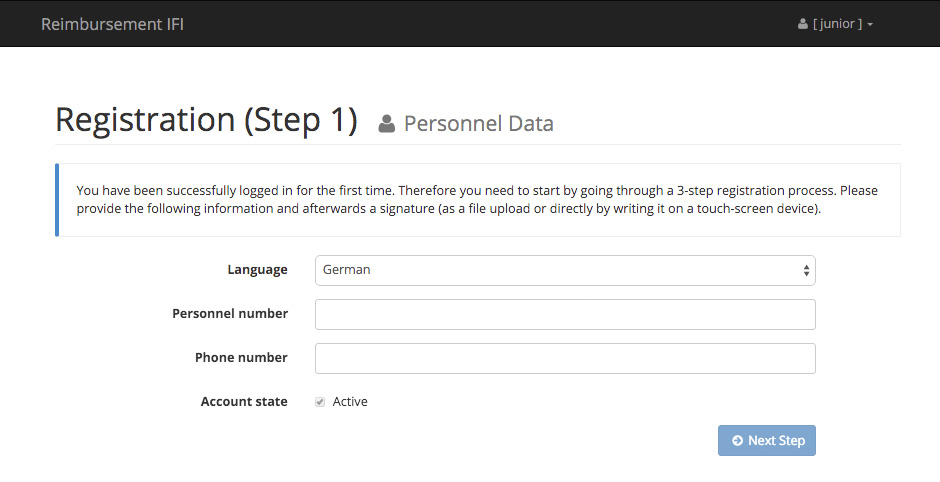
\includegraphics[width=0.80\textwidth]{registration-step01}}
    \caption{Registration step one: Capture personnel data}
    \label{fig:registration-step01}
\end{figure}

\subsection{Step 2}
On Figure \ref{fig:registration-step02} the user needs to add his handwritten signature either by uploading an image or capture it using a third party touchscreen device like a smart phone. This signature is required to sign the generated Pdf document containing all expense items.  

\begin{figure}[H]
    \centering
    \fbox{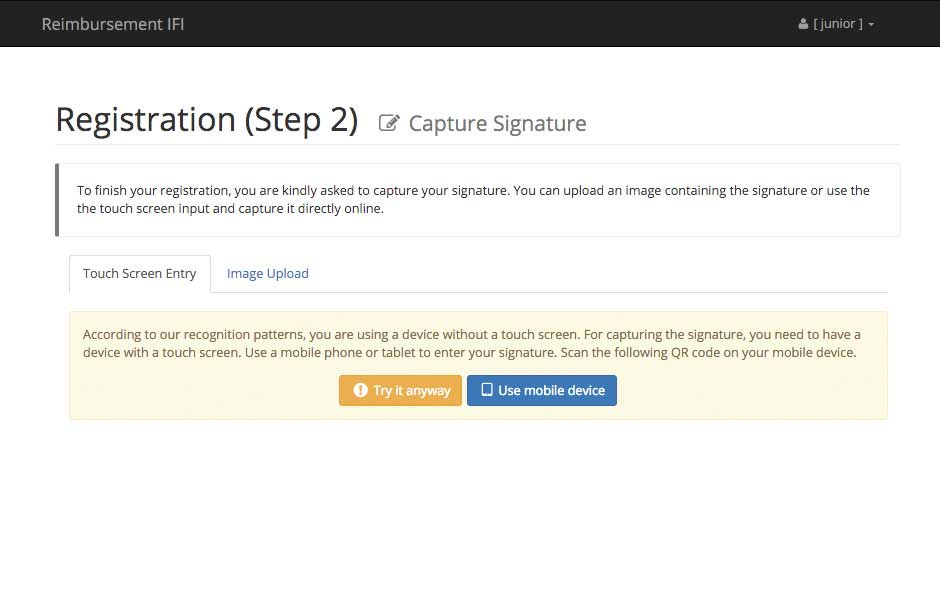
\includegraphics[width=0.80\textwidth]{registration-step02}}
    \caption{Registration step two: Capture signature}
    \label{fig:registration-step02}
\end{figure}

After completing the registration process, these captured information and signature can always be edited by calling the settings screen on the navigation bar.
\clearpage

\section{Expenses}

An expense is an entity captured by an user. Every expense is defined by an \textbf{accounting description} that will be visual in SAP. An expense consists of 1 to 15 receipts.

The user has to create an expense, add receipts to it and assign it to the manager. The manager will check the correctness, add the corresponding projects and assign it to the finance admin if the Expense is correct. For a detailed description of the process please refer to section \ref{sec:process}. 

\subsection{Create expense}

To create an expense, to user needs to navigate to the \textbf{Dashboard} and click on the button \textbf{Create new Expense}. A modal window will open where an SAP description needs to be entered. This value will be used at the SAP system. The SAP description can changed afterwards as well.\newline After you entered the SAP description and clicked \textbf{Next} you will enter the \textit{Expense-View} (Figure \ref{fig:expensesitems-overview}). This view shows all available receipts captured for this specific expense. 

\begin{figure}[H]
    \centering
    \fbox{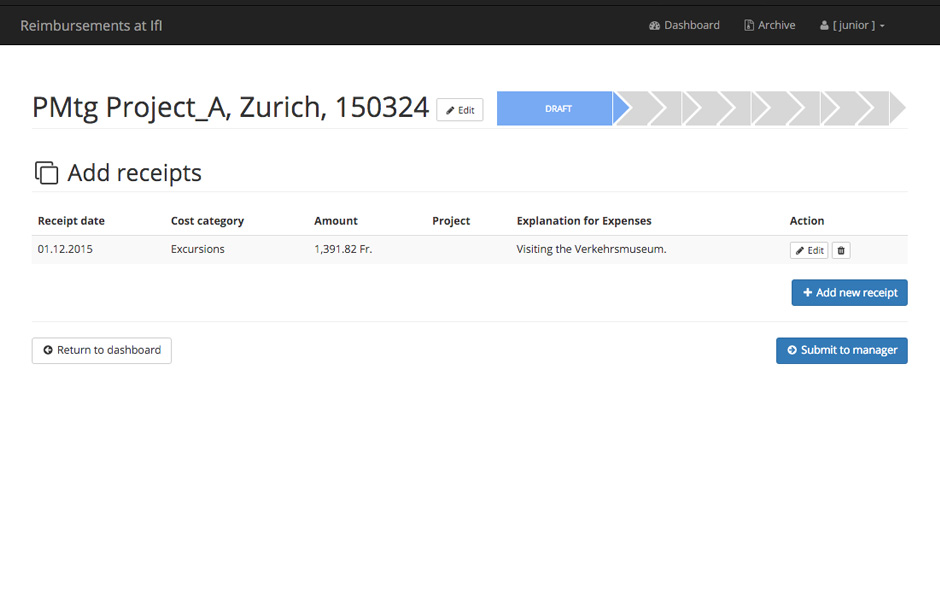
\includegraphics[width=0.80\textwidth]{expensesItems-overview}}
    \caption{Expense-View: Overview}
    \label{fig:expensesitems-overview}
\end{figure}

On the top left-hand side the \textbf{SAP description} is added. The small button on the right can be used to change it. On the top right-hand side the actual process step and the open steps of the Expense are visualized. This process bar always shows the current state the Expense is in, beside the completed and the open ones.\newline
Further the user can add, edit and remove receipts. To add a new receipt the user needs to click on the button \textbf{Add new Receipt}. See Section \ref{sec:addreceipt} for details.\newline
Existing receipts can be edited and removed by clicking on the respective buttons in the receipts-list.


\subsection{Add receipt}
\label{sec:addreceipt}
By adding a new receipt or editing an existing one, the user needs to enter the following mandatory information:  
\begin{itemize}
    \item \textbf{Receipt date} will further be used to calculate the correct exchange rate if a foreign currency is selected.  
    \item \textbf{Cost category} selected out of a defined list of available cost categories.
    \item Original and calculated amount based on the exchange rate.
    \item The \textbf{project assignment} is added by a user with role \textit{manager}, \textit{deputy manager} or \textit{finance administrator}.
    \item A short \textbf{explanation} that describes the purpose of the receipt.   
    \item \textbf{Receipt attachment} used for verification purpose of the captured receipt. 
\end{itemize}

See Figure \ref{fig:expenses-add01} for details.


\begin{figure}[H]
    \centering
    \fbox{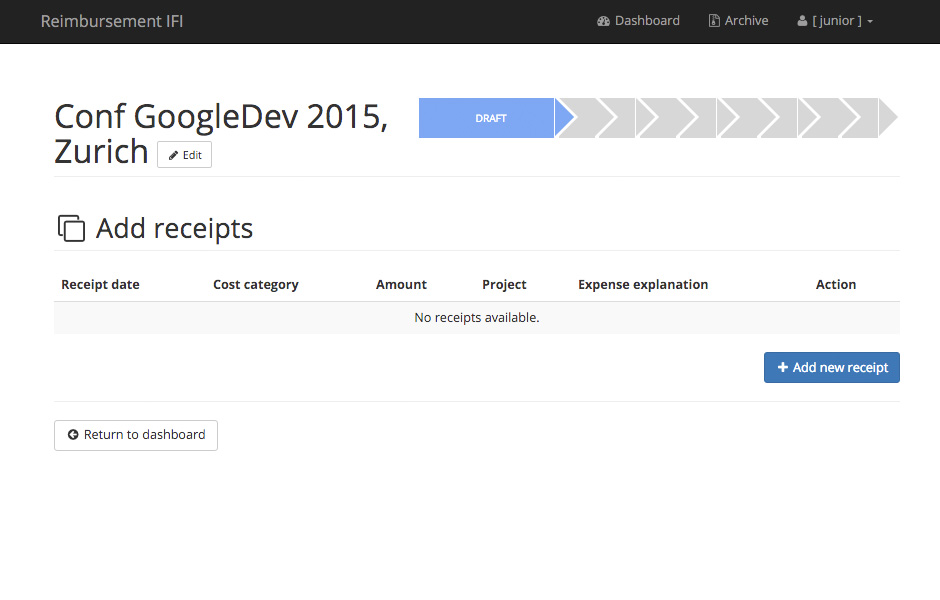
\includegraphics[width=0.80\textwidth]{expenses-add01}}
    \caption{Expense: Add new receipt}
    \label{fig:expenses-add01}
\end{figure}

\subsection{Assign expense to manager}
If all receipts are captured the receipt will be assigned to the manager in charge. After the assignment, the expense cannot be edited anymore. To assign an expense to the manager, click on the \textbf{Submit to Manager} button.

\subsection{States}
Every expense will be in one of the following states during the process:

\begin{itemize}
    \item \textbf{DRAFT} state occurs if the expense is created and it has not been assigned to a \textit{manager}.
    \item \textbf{ASSIGNED} state occurs if a \textit{manager} or \textit{deputy manager} has assigned the expense to him.
    \item \textbf{REJECTED} state occurs if the created expense is not accepted by the \textit{manager}, \textit{deputy manager} or \textit{finance administrator}. In \textbf{REJECTED} status it will be reassigned to the user who created it.
    \item \textbf{SIGNED} state occurs if the expense has been signed by all three instances; \textit{employee}, \textit{manager} or \textit{deputy manager} and \textit{finance administrator}
    \item \textbf{PRINTED} state occurs if the expense and all its receipts are successfully converted into a digital document.
\end{itemize}

\subsection{Digital signature}
tbd

\section{User}

Every user that exists in the LDAP of the University of Zurich is capable to login to the system. He can use the same user name and password that he uses for the other University of Zurich services for login. See Section \ref{sec:registration} for more details.  

There exists different roles for users to login to the system. A user is allowed to have exactely one role out of the four defined. The roles are provided and synchronized with the LDAP-Server of the University of Zurich. The following roles exist in the system:

\begin{itemize}
    \item \textbf{Employees} are authorized to create and edit expenses that they created. However, an expense cannot be edited once it has been assigned to a manger.
    \item \textbf{Managers} are authorized to reject, accept and edit expenses that he assigns to him. A \textit{manager} is also capable of creating expenses and editing them until it has been assigned to a deputy manger.
    \item \textbf{Deputy manager} has the same authorizations as the \textit{manager} for designated \textit{managers} or if a \textit{manager} is outreach.   
    \item \textbf{Finance administrator} is authorized to reject, accept and edit expenses after they have been accepted by a \textit{manager} or \textit{deputy manager}. Furthermore they can manage the available cost categories.
\end{itemize}

\section{Guest view}
With the guest view users can retrieve expenses without the need of an account for the system. They can open the guest view by a special URL, that is provided on every printed expense document. The URL is located on the second page in form of a QR-Code and an URL. The user can either scan the QR-Code or typewrite the URL in a browser window and he'll get access to the respective expense.


\section{Process}
\label{sec:process}
